% !TEX encoding = UTF-8
% !TEX TS-program = pdflatex
% !TEX root = ../tesi.tex

%**************************************************************
\chapter{Integrazione di Amazon Lex}
\label{cap:lex}
%**************************************************************

In questo capitolo viene approfondito lo sviluppo e l'integrazione del \gls{chatbot} vocale per l'interazione tra l'utente e l'applicativo. \\

%**************************************************************

\section{Presentazione del problema}
MariBa è una piattaforma per il salvataggio dei risultati delle partite giocate dai dipendenti di \azienda durante le 
pause pranzo e caffè. \\
Il caricamento di una nuova partita prevede l'inserimento di molti dati contenenti le informazioni rilevanti alle predizioni delle partite successive. 
In particolare viene richiesto: 
\begin{itemize}
	\item \textbf{Calcetto}:
	\begin{itemize}
		\item Autogol effettuati da ciascun giocatore;
		\item Gol effettuati da ciascun giocatore;
	\end{itemize}
	\item \textbf{Mario Kart}:
	\begin{itemize}
		\item Torneo giocato;
		\item Posizione finale di ciascun giocatore;
		\item Punteggio finale di ciascun giocatore.
	\end{itemize}
	\item \textbf{Duck Game}:
	\begin{itemize}
		\item Punteggio di ciascun giocatore.
	\end{itemize}
\end{itemize}
Poiché l'inserimento di questi dati risultava laborioso, è stato richiesto di implementare un \gls{chatbot} vocale 
che permettesse il salvataggio delle partite giocate.
\section{Progettazione}
In questa sezione vengono descritti l'architettura ed il funzionamento del sistema di interazione vocale implementato. \\ 
Inoltre viene presentato il design dell'applicazione web dopo l'integrazione.
	\subsection{Architettura}
	Il micro-servizio sviluppato fa uso dei seguenti servizi messi a disposizione da \gls{AWS}:
	\begin{itemize}
		\item \emph{Amazon Lex};
		\item \emph{Amazon S3};
		\item \emph{AWS Lambda}.
	\end{itemize}
		\subsubsection{Amazon Lex}
		\emph{Amazon Lex} è un servizio di intelligenza artificiale completamente gestito che mette a disposizione 
		modelli avanzati di linguaggio naturale per permettere lo sviluppo di interfacce di comunicazione all'interno 
		di applicazioni software. Nel progetto di stage è stata utilizzata la verisone due di \emph{Amazon Lex} per 
		implementare un \gls{chatbot} vocale per interagire con l'applicazione e registrare i risultati delle partite 
		giocate. \\
		
		\noindent La creazione di \gls{chatbot} con \emph{Amazon Lex} può essere effettuata attraverso l'utilizzo della console messa a disposizione da \gls{AWS}. \\
		Per ogni \gls{chatbot} di \emph{Lex} possono essere definiti diversi \emph{intent}, ovvero azioni che si
		vuole portare a termine attraverso l'utilizzo dello stesso. In ciascun \emph{intent} possono essere definiti:
		\begin{itemize}
			\item \textbf{Frasi d'esempio}: frasi che l'utente deve pronunciare al \gls{chatbot} per richiamare uno
			specifico \emph{intent}. Nella console vengono inserite alcune frasi rappresentative e successivamente \emph{Lex} sarà in grado di comprenderne delle varianti; 
			\item \textbf{Slot}: variabili a cui il \gls{chatbot} assegnerà un valore sulla base
			dell'input fornitogli dall'utente. Gli slot sono tipizzati:	\emph{Lex} mette a disposizione alcuni tipi built-in ma permette anche di definire tipi personalizzati;
			\item \textbf{Flusso della conversazione}: con quale ordine chiedere all'utente il valore degli \emph{slot} necessari e quali frasi usare per farlo.		
		\end{itemize}
		
		\noindent Inoltre, per effettuare delle validazioni sull'input, \emph{Lex} include la possibilità di associare al \gls{chatbot} una funzione \emph{Lambda} da richiamare alla fine di un \emph{intent} oppure ogni volta che viene fornito un valore per uno \emph{slot}. \\
		
		\noindent Per la realizzazione del prodotto sono state utilizzate le seguenti funzioni di \emph{Lex}:
		\begin{itemize}
			\item \texttt{RecognizeUtterance}: invia l'input (audio o testo) dell'utente ad \emph{Amazon Lex}. Quest'ultimo interpreta l'input utilizzando i modelli di machine learning costruiti per il \gls{chatbot};
			
			\item \texttt{PutSession}: permette di modificare lo stato della \emph{sessione} creata quando un utente inizia la conversazione con il \gls{chatbot}. Tale sessione è identificata attraverso il \emph{sessionId} (assegnato automaticamente o specificato manualmente). 
		\end{itemize}
		
		\subsubsection{Amazon S3}
		\emph{Amazon Simple Storage Service} (S3) è un servizio di archiviazione oggetti. Al suo interno i dati sono 
		organizzati in \emph{bucket}. All'interno di ogni \emph{bucket} è possibile definire dei prefissi per poter 
		organizzare al meglio gli oggetti caricati (simile al concetto di ``cartella''). \\ 
		Per evitare un passaggio diretto degli audio tra front-end e back-end si è utilizzato un \emph{bucket}. S3 
		infatti fornisce la possibilità di generare un URL per effettuare operazioni di \emph{upload} o 
		\emph{download} in una specifica posizione all'interno del \emph{bucket} senza necessità di autenticazione. \\ 
		In particolare, per generare l'URL per l'upload viene effettuata la seguente operazione:
		
		\begin{figure}[H]
			\centering
			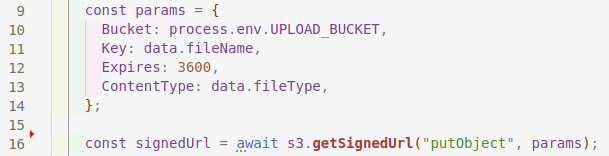
\includegraphics[width=11cm]{immagini/getURL.png} \\
			\caption{\label{fig:getURLAudio} Snippet di codice per ottenere l'URL presigned}
		\end{figure}
		
		Nel codice sopra riportato:
		\begin{itemize}
			\item \textbf{Bucket}: nome del \emph{bucket} su cui effettuare l'operazione;
			\item \textbf{Key}: nome del file che si vuole caricare con il presigned che si ottiene, specificando eventuali prefissi;
			\item \textbf{ContentType}: tipo del file che si vuole caricare. Nel caso degli audio registrati da MariBa, il formato è \emph{audio/wav};
			\item \textbf{``putObject''}: tipo di operazione che si vuole effettuare con l'URL generato. In questo caso si tratta di un'operazione PUT.
		\end{itemize}
		
		Gli audio caricati hanno utilità molto breve: infatti una volta che il back-end ne ha effettuato il \emph{download}, 
		essi non verranno più utilizzati. Di conseguenza, per evitare di lasciare all'interno del \emph{bucket} dell'inutile spazzatura, è stata impostata una \emph{lifecycle rule} in modo tale che tutti gli audio caricati (con prefisso \emph{audio/}) vengano eliminati in modo automatico dopo un giorno dal loro caricamento. \\
		
		\noindent  L'operazione eseguita per generare l'URL per il download è molto simile a quella sopra riportata con la sola differenza che \emph{``putObject''} viene sostituito con \emph{``getObject''}.
	
		\subsubsection{AWS Lambda}
		Di seguito sono descritte le funzioni \emph{Lambda} implementate per il funzionamento del \gls{chatbot} \emph{Lex}:
		\begin{itemize}
			\item \texttt{getPresignedUpload}: richiede il presigned URL per il caricamento dell'audio;
			
			\item \texttt{elaborateAudio}: effettua la chiamata effettiva a \emph{Lex} specificando il \gls{chatbot} da utilizzare. In particolare:
			\begin{enumerate}
				\item Scarica l'audio dell'utente da \emph{S3};
				\item Chiama \texttt{lex.RecognizeUtterance} sull'audio ottenuto;
				\item \texttt{lex.RecognizeUtterance} restituisce l'audio contenente la risposta del \gls{chatbot};
				\item Carica l'audio di risposta su \emph{S3};
				\item Restituisce al front-end le informazioni sulla posizione nel bucket dell'audio di risposta.
			\end{enumerate}
			
			\item \texttt{maribaBot}: funzione utilizzata dal bot per la validazione dell'input e/o alla conclusione di un intent. \\
			In particolare, la funzione controlla che i giocatori inseriti dall'utente siano effettivamente presenti all'interno del database:
			\begin{itemize}
				\item Poiché i nickname sono una trascrizione dell'audio ricevuto dall'utente, è stata utilizzata la 
				\gls{distanza di Levenshtein} per fare in modo che non fosse necessaria una corrispondenza perfetta 
				con il nickname salvato;
				\item Quando viene effettuato tale controllo, viene tenuto come definitivo il nickname con \gls{distanza di Levenshtein} minore;
				\item  Nel caso in cui non fossero presenti nel database nickname con \gls{distanza di Levenshtein} minore di tre rispetto a quello inserito, il nickname viene considerato come non valido e lo slot corrispondente viene chiesto nuovamente all'utente.
			\end{itemize}
		
			\item \texttt{getPresignedDownloadAudio}: richiede il presigned URL per il download dell'audio da \emph{S3}.
			
		\end{itemize}
		
	\subsection{Funzionamento generale}
	
	\noindent Nel \gls{chatbot} implementato durante lo stage sono stati definiti diversi \emph{intent}. Infatti, per ciascun gioco disponibile su MariBa sono stati implementati due \emph{intent}:
	\begin{itemize}
		\item Uno per l'inserimento dei giocatori;
		\item Uno per l'inserimento dei risultati della partita.
	\end{itemize}
	Inoltre, sono stati definiti i seguenti slot:
	\begin{itemize}
		\item Uno per ciascun giocatore;
		\item Uno per ciascun dato richiesto nel salvataggio della partita nell'interfaccia grafica di MariBa.
	\end{itemize}
	
	\noindent Pronunciando ad esempio ``Voglio registrare una partita a Mario Kart'' il \gls{chatbot} capirà l'intenzione
	dell'utente e inizierà chiedendo quali siano i giocatori partecipanti. Una volta concluso l'inserimento dei
	nominativi, verrà richiamato automaticamente il secondo \emph{intent} per permettere l'inserimento dei risultati. \\
	
	\noindent Il funzionamento generale dell'applicazione è riportato nella \autoref{fig:funzionamento-lex} e descritto di seguito.
	
	\begin{figure}[H]
		\centering
		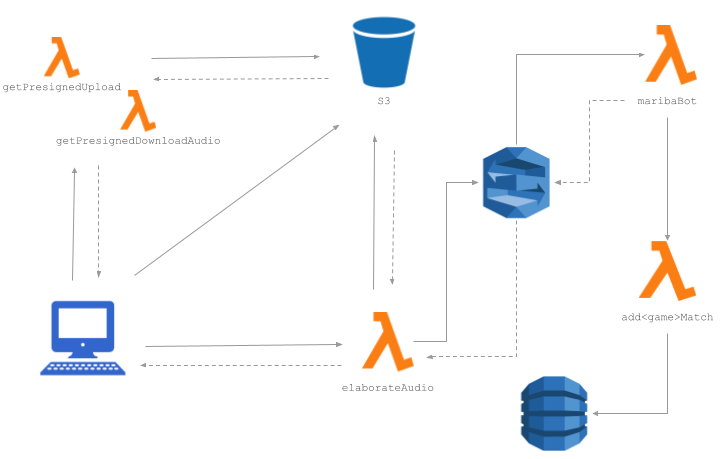
\includegraphics[width=12cm]{immagini/funzionamentoLex.png} \\
		\caption{\label{fig:funzionamento-lex} Grafico del funzionamento del chatbot}
	\end{figure}

	\begin{enumerate}
		\item L'utente registra un audio attraverso l'apposita interfaccia all'interno del sito MariBa;
		\item Il front-end utilizza la funzione \texttt{getPresignedUpload} per ottenere l'URL per il caricamento dell'audio nel \emph{bucket} di \emph{S3};
		\item Una volta ottenuto il link, il front-end procede al caricamento;
		\item Chiama la funzione \texttt{elaborateAudio} e attende il completamento della sua esecuzione;
		\item \texttt{elaborateAudio} scarica l'audio dal \emph{bucket} e lo invia a \emph{Lex} per l'elaborazione;
		\item \emph{Lex} utilizza \texttt{maribaBot} per la validazione delle informazioni estratte dall'audio e restituisce a sua volta un audio contenete la risposta generata dal \gls{chatbot};
		\item \texttt{elaborateAudio} carica la risposta su \emph{S3} e restituisce le informazioni sulla posizione dell'oggetto all'interno del \emph{bucket} al front-end;
		\item Il front-end chiama la funzione \texttt{getPresignedDownloadAudio} per ottenere l'URL per il \emph{download} dell'audio;
		\item L'audio viene scaricato e viene riprodotto;
		\item Quando viene confermato il salvataggio di una partita, \texttt{maribaBot} procede al caricamento nel database dei dati estrapolati dalla conversazione con l'utente utilizzando la corretta funzione \emph{Lambda} a seconda del gioco utilizzato.
	\end{enumerate}
	
	\subsection{Design dell'interfaccia}
	Per il design dell'interfaccia, prima della sua effettiva codifica, sono stati realizzati dei \emph{wireframes} utilizzando \emph{Balsamiq}. In questo modo si è potuto definire il flusso di funzionamento a livello di front-end. \\ 
	
	\noindent Successivamente, la realizzazione dell'interfaccia è avvenuta utilizzando \emph{Angular 12.x} in combinazione con la libreria 
	\emph{Nebular}, specifica per lo sviluppo di interfacce utente. \\
	
	\noindent Per l'utilizzo del \gls{chatbot} vocale è stato integrato all'interno dell'header del sito un pulsante.
	Tenendo premuto tale pulsante è possibile registrare l'audio contenente le richieste desiderate. Per aiutare l'utente
	sono stati inseriti alcuni \emph{tooltip} contenenti consigli su frasi da pronunciare o su come iniziare una registrazione.
	
	\begin{figure}[H]
		\centering
		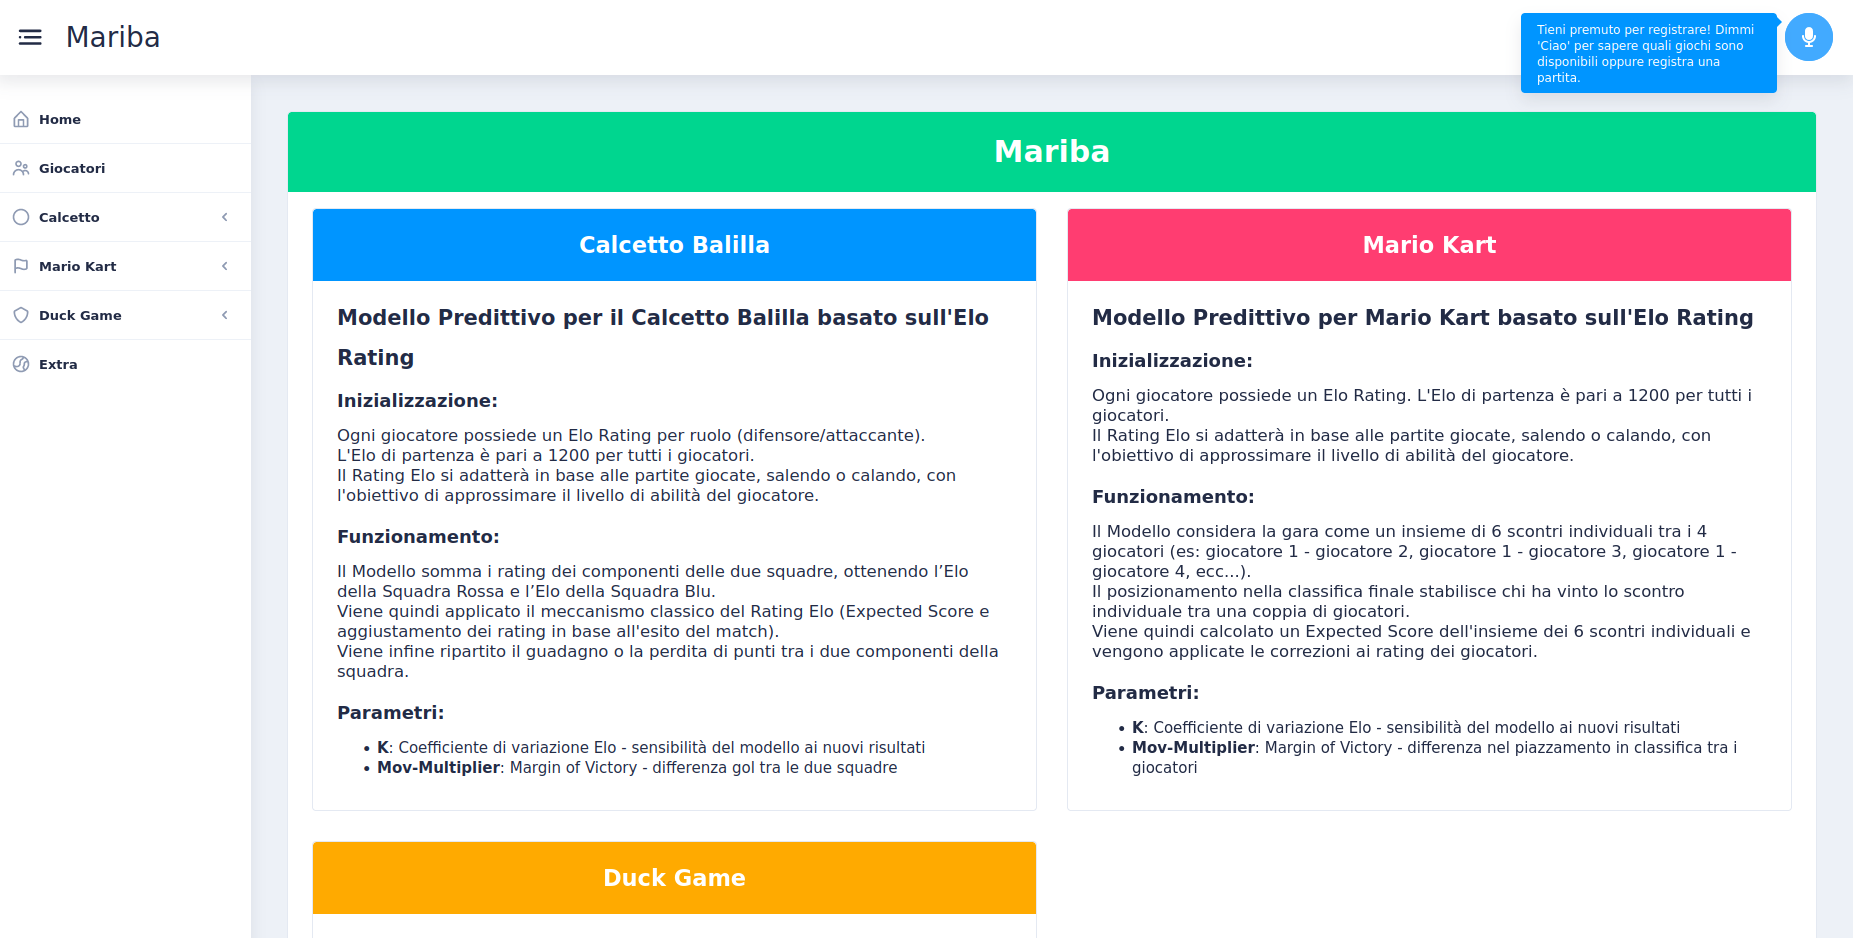
\includegraphics[width=\textwidth]{immagini/pulsanteStart.png} \\
		\caption{\label{fig:audio-start} Schermata iniziale con integrazione del chatbot}
	\end{figure}
	
	\bigskip

	\noindent L'aspetto del pulsante varia a seconda dello stato della conversazione:
	
	\paragraph{Stato iniziale}  ~\smallskip 
	
	\noindent L'applicativo è pronto per l'inizio di una nuova conversazione. 
	
	\begin{figure}[H]
		\centering
		
\includegraphics[width=1.5cm]{immagini/stato_iniziale.png} \\
		\caption{\label{fig:stato-iniziale} Stato iniziale del pulsante di registrazione}
	\end{figure}

	\paragraph{In registrazione}  ~\smallskip 
	
	\noindent L'applicativo sta registrando l'audio. 
	
	\begin{figure}[H]
		\centering
		
\includegraphics[width=1.4cm]{immagini/registrazione.png} \\
		\caption{\label{fig:registrazione} Pulsante nella fase di registrazione}
	\end{figure}
	
	
	\paragraph{Elaborazione dell'audio}  ~\smallskip 
	
	\noindent L'applicativo sta procedendo all'invio dell'audio per l'elaborazione. 
	
	\begin{figure}[H]
		\centering
		
\includegraphics[width=1.5cm]{immagini/elaborazione.png} \\
		\caption{\label{fig:elaborazione} Pulsante nella fase di elaborazione}
	\end{figure}
	
	
	\paragraph{Riproduzione dell'audio ricevuto da Lex}  ~\smallskip 
	
	\noindent L'applicativo sta riproducendo l'audio ricevuto in risposta dal \gls{chatbot}.
	
	\begin{figure}[H]
		\centering
		
\includegraphics[width=1.5cm]{immagini/riproduzione.png} \\
		\caption{\label{fig:riproduzione} Pulsante nella fase di riproduzione dell'audio}
	\end{figure}
	 

	\paragraph{Pronto per la registrazione della risposta}  ~\smallskip 
	
	\noindent L'applicativo è pronto per la registrazione da parte dell'utente della prossima interazione con il \gls{chatbot}. 
	
	\begin{figure}[H]
		\centering
		
\includegraphics[width=2.4cm]{immagini/risposta.png} \\
		\caption{\label{fig:risposta} Pulsante indica che il chatbot aspetta una risposta dall'utente}
	\end{figure}
	
	\paragraph{Stato di errore} ~\smallskip 
	
	\noindent In caso di errore nell'elaborazione dell'audio viene mostrato a schermo un \emph{pop-up}.
	
		\begin{figure}[H]
			\centering
			
\includegraphics[width=5cm]{immagini/errore_reg.png} \\
			\caption{\label{fig:errore-reg} Errore nell'elaborazione dell'audio}
		\end{figure}
	
